\documentclass[landscape,12pt]{article}
\usepackage[letterpaper,margin=0.6in]{geometry}
\usepackage[T1]{fontenc}
\usepackage{lmodern}
\usepackage{microtype}
\usepackage{amsmath,amssymb}
\usepackage{booktabs}
\usepackage{array}
\usepackage{xcolor}
\usepackage{tikz}
\usetikzlibrary{arrows.meta,positioning,fit,backgrounds}
\usepackage{titlesec}
\usepackage{enumitem}
\setlist[itemize]{leftmargin=1.3em,itemsep=2pt,topsep=3pt}
\pagestyle{empty}
\emergencystretch=3em

\definecolor{bench}{HTML}{1B5E20}
\definecolor{solver}{HTML}{0D47A1}
\definecolor{phys}{HTML}{B71C1C}
\definecolor{prior}{HTML}{8D6E00}
\definecolor{soft}{HTML}{F5F5F5}

\newcommand{\pagehead}[2]{%
  {\Large\bfseries #1}\\[1pt]
  {\small\itshape #2}\\[-4pt]
  \rule{\linewidth}{0.6pt}\\[4pt]}

\begin{document}

% ================================================== PAGE 1
\pagehead{Where your bench data enters the model}%
{Hunter Kinder --- proposed Phase 1 collaboration. One page of architecture, one of protocol, one of data handling.}

\vspace{2pt}
\begin{center}
\scalebox{1.18}{%
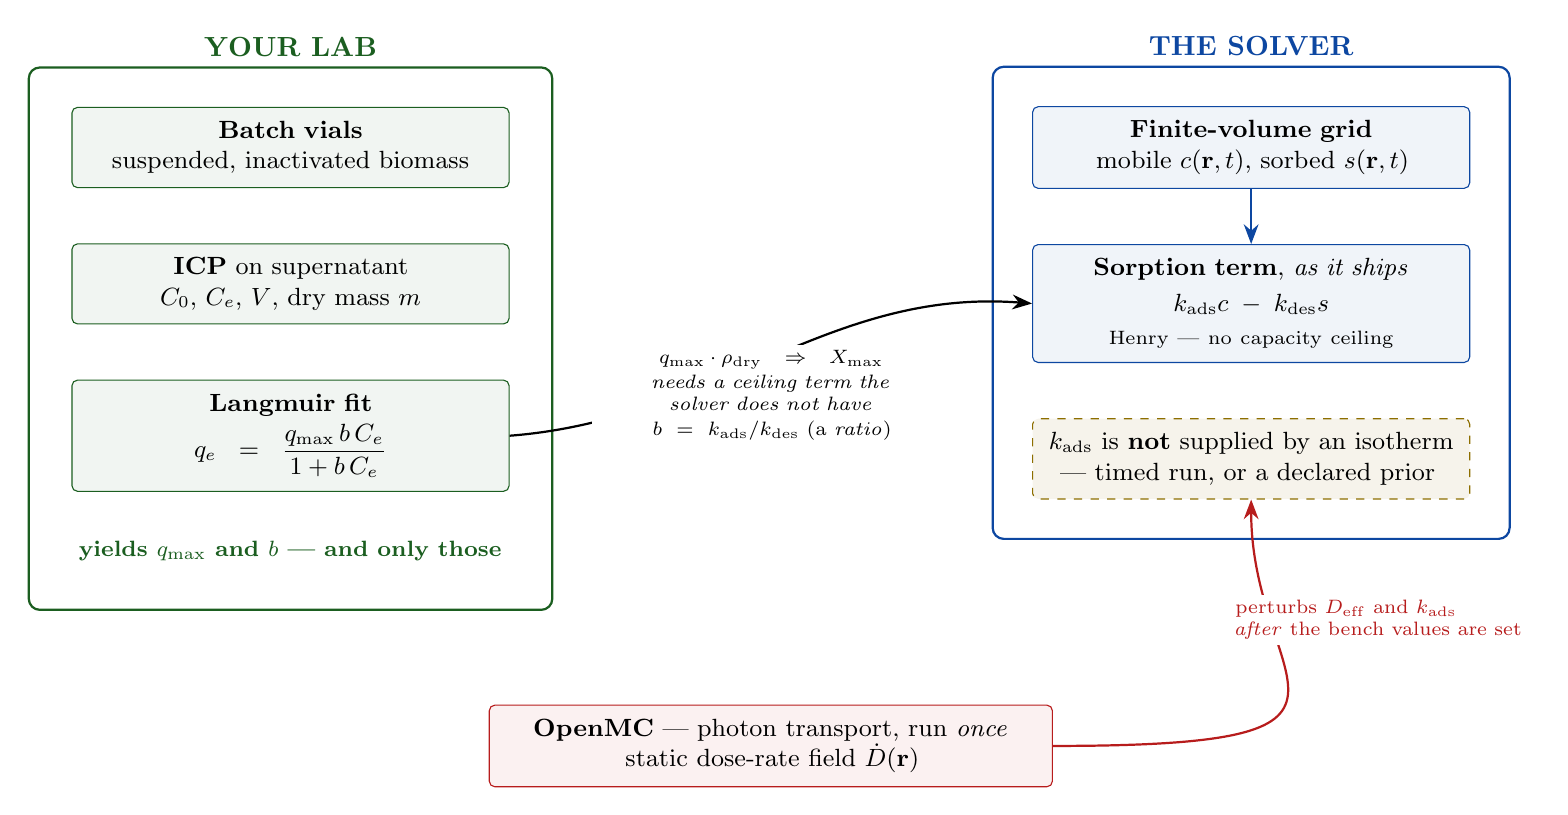
\begin{tikzpicture}[
  font=\small, scale=1.0,
  box/.style={draw,rounded corners=2pt,align=center,inner sep=5pt,
              minimum height=9mm,text width=52mm},
  lab/.style={box,draw=bench,fill=bench!6},
  sol/.style={box,draw=solver,fill=solver!6},
  rad/.style={box,draw=phys,fill=phys!6,text width=68mm},
  pri/.style={box,draw=prior,dashed,fill=prior!8},
  ar/.style={-{Stealth[length=2.5mm]},thick},
]

% ---- left: the bench
\node[lab] (vial) at (0,0) {\textbf{Batch vials}\\suspended, inactivated biomass};
\node[lab,below=7mm of vial] (icp) {\textbf{ICP} on supernatant\\$C_0$,\ $C_e$,\ $V$,\ dry mass $m$};
\node[lab,below=7mm of icp] (iso) {\textbf{Langmuir fit}\\[2pt]$q_e = \dfrac{q_{\max}\,b\,C_e}{1+b\,C_e}$};
\node[below=5mm of iso,text=bench,font=\bfseries\footnotesize,text width=54mm,align=center]
     (out1) {yields $q_{\max}$ and $b$ --- and only those};

% ---- right: the solver
\node[sol] (grid) at (12.2,0) {\textbf{Finite-volume grid}\\mobile $c(\mathbf{r},t)$, sorbed $s(\mathbf{r},t)$};
\node[sol,below=7mm of grid] (sink) {\textbf{Sorption term}, \emph{as it ships}\\[2pt]$k_{\mathrm{ads}}c - k_{\mathrm{des}}s$\\[1pt]{\scriptsize Henry --- no capacity ceiling}};
\node[pri,below=7mm of sink] (kads) {$k_{\mathrm{ads}}$ is \textbf{not} supplied by an
  isotherm --- timed run, or a declared prior};

% ---- the transfer, routed above the gap
\draw[ar] (iso.east) .. controls +(2.6,0.2) and +(-2.6,0.2) .. (sink.west);
\node[font=\scriptsize,align=center,text width=44mm,fill=white,inner sep=2pt] at (6.1,-3.15)
  {$q_{\max}\!\cdot\!\rho_{\mathrm{dry}}\ \Rightarrow\ X_{\max}$\\[1pt]
   {\itshape needs a ceiling term the solver does not have}\\[1pt]
   $b = k_{\mathrm{ads}}/k_{\mathrm{des}}$ (a \emph{ratio})};
\draw[ar,solver] (grid) -- (sink);

% ---- radiation layer, well clear of both groups
\node[rad] (mc) at (6.1,-7.6) {\textbf{OpenMC} --- photon transport, run \emph{once}\\
  static dose-rate field $\dot{D}(\mathbf{r})$};
\draw[ar,phys] (mc.east) .. controls +(4.6,0) and +(0,-2.4) .. (kads.south);
\node[font=\scriptsize,align=left,text=phys,text width=38mm,fill=white,inner sep=2pt] at (13.9,-6.0)
  {perturbs $D_{\mathrm{eff}}$ and $k_{\mathrm{ads}}$\\\emph{after} the bench values are set};

\begin{scope}[on background layer]
  \node[fit=(vial)(iso)(out1),draw=bench,thick,rounded corners,
        inner sep=5mm,label={[text=bench,font=\bfseries]above:YOUR LAB}] {};
  \node[fit=(grid)(kads),draw=solver,thick,rounded corners,
        inner sep=5mm,label={[text=solver,font=\bfseries]above:THE SOLVER}] {};
\end{scope}
\end{tikzpicture}}
\end{center}

\vspace{-1mm}
{\small
\textbf{The point of the split.} The sorption capacity is a property of the biomass and is
measured with no radiation present. The dose field is computed once and never reads the
concentration back. So the bench numbers are fixed before the physics runs, and the physics
can only scale them --- \emph{by construction, because the codes are run in that order}. That
is a design choice I am declaring, not a law: at high metal loading the assumption weakens,
and the manuscript says where.

\textbf{What I am asking you to help me measure is a sponge.} Not radiotrophy, not a survival
effect --- an equilibrium capacity.}

\newpage
% ================================================== PAGE 2
\pagehead{Phase 1: the bench assay}%
{A standard batch biosorption isotherm. Finite, bounded, and using material you already have.}

\vspace{1mm}
\begin{minipage}[t]{0.485\linewidth}
{\large\bfseries\color{bench} Material}
\begin{itemize}
  \item Whatever biomass your lab already grows in excess --- I am not asking you to
        establish a new culture.
  \item \textbf{Inactivated.} Biosorption is metabolically independent, so dead or
        heat-killed biomass is standard in this literature. That removes viability
        maintenance from the first experiment. Heat, not azide --- see the control below.
  \item Suspended, not a coupon. A coupon measures capacity and diffusion at the same time
        and resolves neither; the suspended assay isolates the thermodynamic limit.
\end{itemize}

\vspace{2mm}
{\large\bfseries\color{bench} Controls}
\begin{itemize}
  \item \textbf{Abiotic blank} --- vessel plus solution, no biomass. Wall loss and
        adsorption to glassware are otherwise counted as uptake.
  \item \textbf{Metabolic control} --- a temperature shift, \emph{not} sodium azide. Azide
        is a ligand that complexes transition metals and shifts speciation, confounding the
        measurement it is meant to control.
  \item \textbf{Blank carried through the identical handling}, including the same
        de-watering and the same delay before weighing.
\end{itemize}
\end{minipage}\hfill
\begin{minipage}[t]{0.485\linewidth}
{\large\bfseries\color{bench} Quality checks}
\begin{itemize}
  \item \textbf{Aggregation state} --- flow cytometry to confirm the suspension is
        monodisperse. Clumping reduces accessible surface and shows up as a lower
        $q_{\max}$ that is an artefact of handling.
  \item \textbf{The normaliser's own variance, measured first.} Wet/dry ratio across
        replicates of one biomass, reported as a CV. If that is 20\%, dry mass is not a
        usable normaliser and knowing so early is worth more than a careful number nobody
        can reproduce.
  \item \textbf{Detectability before replication.} A biomass mass under the blank's noise is
        a substrate problem, and no replicate count fixes it --- so that test comes first,
        then the CV, then the replicate number.
\end{itemize}

\vspace{2mm}
{\large\bfseries\color{bench} Deliverable}
\begin{itemize}
  \item A paired $[C_e,\ q_e]$ array from your ICP, with
        $q_e = (C_0 - C_e)V/m$, plus the blanks and the CV.
\end{itemize}
\end{minipage}

\vspace{3mm}
\noindent\rule{\linewidth}{0.4pt}\\[2pt]
{\small\textbf{Fixed procedure, because these dominate reproducibility more than anything
else on this page:} one separation method at a fixed vacuum or RCF; a fixed duration; a fixed
elapsed time from separation to balance, since evaporation begins immediately and two minutes
is a real mass difference; a stated drying temperature with an explicit constant-weight
criterion rather than ``dried to constant weight''. \emph{Drying temperature is the one I would
rather take from you than propose} --- 105\,\textdegree C is the total-solids convention but
can char organics, and gentler drying or lyophilisation is common for biomass. That is a
question with a house answer.}

\newpage
% ================================================== PAGE 3
\pagehead{From your number to my parameter}%
{What the measurement becomes, and what it is still not.}

\vspace{1mm}
\begin{minipage}[t]{0.45\linewidth}
{\large\bfseries\color{solver} Where the number would land}\\[3pt]
The isotherm gives capacity per unit \emph{mass}:
\[ q_e = \frac{q_{\max}\,b\,C_e}{1+b\,C_e}\quad\text{[mg\,g$^{-1}$]} \]
The solver tracks mass per unit \emph{volume}, so:
\[ \boxed{\,X_{\max} = q_{\max}\cdot\rho_{\mathrm{dry}}\,} \]
\emph{This is not yet a bridge.} The sorption term that ships is linear in $c$ with no
capacity ceiling, so there is no $X_{\max}$ in the code for this number to enter. Adding
one is a declared model change, not a plug-in.

\vspace{2mm}
{\large\bfseries\color{prior} Two things this does not give me}\\[3pt]
\textbf{1. A rate.} $b$ is thermodynamic --- at equilibrium it is the \emph{ratio}
$k_{\mathrm{ads}}/k_{\mathrm{des}}$, and infinitely many rate pairs share one ratio. If the
solver needs $k_{\mathrm{ads}}$, that requires timed sampling of the same vial; otherwise it
is carried as an unmeasured prior and labelled one.

\vspace{2mm}
\textbf{2. A biofilm number.} Suspended and biofilm biomass differ in EPS composition, surface
charge and accessible sites. This is a \emph{bound and a starting value}, not a transferable
parameter --- and the gap between them is itself measurable in Phase 2.

\end{minipage}\hfill
\begin{minipage}[t]{0.51\linewidth}
{\large\bfseries\color{solver} Epistemic class travels with the number}\\[3pt]
{\footnotesize
\begin{tabular}{@{}>{\raggedright\arraybackslash}p{2.5cm}>{\raggedright\arraybackslash}p{3.4cm}>{\raggedright\arraybackslash}p{4.6cm}@{}}
\toprule
\textbf{Quantity} & \textbf{Class} & \textbf{Why} \\
\midrule
$q_{\max}$, $b$ & \textcolor{bench}{\textbf{Measured}} (suspended basis) & Phase 1 output, on your ICP \\[2pt]
$\rho_{\mathrm{dry}}$ & \textcolor{prior}{\textbf{Prior}} & Needs paired hydrated volume; Phase 2 \\[2pt]
$X_{\max}$ & \textcolor{prior}{\textbf{Prior}} & \emph{Product inherits the weaker class} \\[2pt]
$k_{\mathrm{ads}}$ & \textcolor{prior}{\textbf{Prior}} & Not obtainable from an isotherm \\[2pt]
$D_{\mathrm{eff}}$ & \textcolor{solver}{\textbf{Phase 2}} & Diffusion cell, biofilm on membrane \\[2pt]
$\lambda$ (radiation) & \textcolor{phys}{\textbf{Uncalibrated}} & The only free parameter left \\
\bottomrule
\end{tabular}}

\vspace{3mm}
{\small A derived quantity cannot be stronger than its weakest input. $X_{\max}$ is built from
a measurement and a prior, so it enters the solver \emph{as a prior} and is reported that way.
Recording that when the number is produced --- rather than when someone asks why the biofilm
does not match --- is the whole discipline.}

\vspace{3mm}
\rule{\linewidth}{0.4pt}\\[3pt]
{\small\textbf{Phase 2, for context only:} biofilm on membrane in a two-chamber diffusion
cell. It is interpretable \emph{because} Phase 1 fixed capacity independently --- the
difference is then attributable to transport rather than confounded with it. That is the
reason for doing these in this order, and the reason Phase 1 is small.}
\end{minipage}

\end{document}
